\documentclass[11pt,a4j,notitlepage]{jsarticle}
\usepackage{TUSGradThesis}

\usepackage[dvipdfmx]{graphicx}
\usepackage[dvipdfmx]{color}
\usepackage{amsmath,amssymb}
\usepackage{setspace}
\usepackage{fancyhdr}
\usepackage{amsmath}
\usepackage{bm}
\usepackage{here}
\usepackage{multirow}
\usepackage{ascmac}
\usepackage[dvipdfmx]{color}
\usepackage{subfigure}
\usepackage{cases}
\usepackage{setspace}
\usepackage{subfiles}
\usepackage{algorithm}
\usepackage{algorithmic}
\usepackage{afterpage}
\usepackage{comment}

\makeatletter
    \renewcommand{\theequation}{%
    \thesection.\arabic{equation}}
    \@addtoreset{equation}{section}
    \def\thefigure{\thesection.\arabic{figure}}
    \@addtoreset{figure}{section}
    \renewcommand{\thetable}{%
    \thesection.\arabic{table}}
    \@addtoreset{table}{section}
\makeatother

\renewcommand\bibname{参考文献}
\newcommand{\Figref}[1]{図~\ref{#1}}
\newcommand{\Eqref}[1]{式~(\ref{#1})}
\newcommand{\Tabref}[1]{表~\ref{#1}}

\newcommand{\mymax}{\mathop{\rm max}\limits}

\makeatletter
\renewcommand{\l@figure}{\@dottedtocline{1}{1.5em}{3.2em}}
\makeatother

\makeatletter
\renewcommand{\l@table}{\@dottedtocline{1}{1.5em}{3.2em}}
\makeatother

\makeatletter
\newcommand{\subsubsubsection}{\@startsection{paragraph}{4}{\z@}%
  {1.0\Cvs \@plus.5\Cdp \@minus.2\Cdp}%
  {.1\Cvs \@plus.3\Cdp}%
  {\reset@font\normalsize\bfseries}
}
\makeatother
\setcounter{secnumdepth}{4}

\setstretch{1.0}
\setcounter{tocdepth}{2}
%\setcounter{secnumdepth}{3}

% 表紙情報
\発表年度{2021} % 全角で書くこと
\著者情報{4618023}{北田 来人}
\指導教員{藤井 孝藏 教授,立川 智章 准教授}{松尾 裕一 教授, 浅田 健吾 助教}
\論文題目{多目的進化計算における}{設計変数の削減方法に関する研究}
{Research of reducing decision variables}{in Multi Objective Evolutionary Algorithm}
\pagestyle{empty}
% 要旨
%\要旨{}
\begin{document}
% 表紙の出力
\begin{center}
\LARGE{多目的進化計算における設計変数の削減方法に関する研究}
\end{center}
\begin{flushright}
北田来人 (藤井 孝藏 教授,立川 智章 准教授, 松尾 裕一 教授, 浅田 健吾 助教)
\end{flushright}
\vspace{-1.75zh}
\section {はじめに}
近年,進化計算は数値最適化,組合せ最適化,制約最適化など様々な場面で利用されている.
実問題においても進化計算が利用されている.
実問題では,計算資源や計算時間に制約ある一方で,考慮するべき評価指標(目的関数)だけでなく設計変数の数が増大する傾向にある.
例えば,複数車体同時最適化問題では,計200変数以上が使用されている.
多目的進化計算では,目的関数の数が増大するとNSGA-IIなどで用いられるパレート支配に基づく優劣評価では進化が進まないという課題がある.(例えば目的関数の数が20を超え始めると,1000個の解を用意してもパレート最適解がほぼ存在しなくなる\cite{Sato1})
また,目的関数空間を幅広く探索するためには多くの集団サイズが必要とされる.さらに実問題では多くの制約条件を考慮しなければならないことがあるが,それらすべての制約を満足する解を探索することは容易ではない.一部に満足することが非常に難しい制約が含まれている場合もある.

上記の問題については,近年の研究により有効な手法が提案されてきている.
1つ目の課題に関しては目的関数の削減をするアプローチ\cite{Deb1}やパレート支配の概念を拡張して解集団をより細かいところまでみて優劣付けするアプローチ\cite{HSato}などのさまざまな研究が行われている,2つ目の課題に関しても例えば,第一段階で全ての制約条件を満たす解を差分進化で抽出し,第二段階でその抽出した解から制約条件をより多く満たす上位$x\%$(xはユーザが決める基準値)の解を局所探索アルゴリズムで見つける\cite{Yo}このような2段階探索などの工夫を行い多数目的かつ強制約問題の最適化に対応でき始めている.

一方,設計変数の数が多い場合の研究はまだ十分行われていない.
図1.1は同じパレートフロントを持つ問題において設計変数の数の違いによる評価値の推移図である.
横軸は目的関数の評価回数(Number of Fitness Evaluation, NFE),縦軸は多目的最適化の評価指標であるパレートフロントのIGD(Inverted Generational Distance)で値が小さいほど収束性と多様性に優れている.
図から,設計変数の数が多くなるにつれて最適化が遅くなっていることがわかる.
そこで本研究では,設計変数が多い問題に対しても効果的な進化計算手法を検討することを目的とする.
ここでは主成分分析に注目し,設計変数空間で主成分分析を行い,縮約された空間で解を生成することで効率的な探索を行う手法を提案することを目的とする.
\begin{figure}[htbp]
\begin{center}
  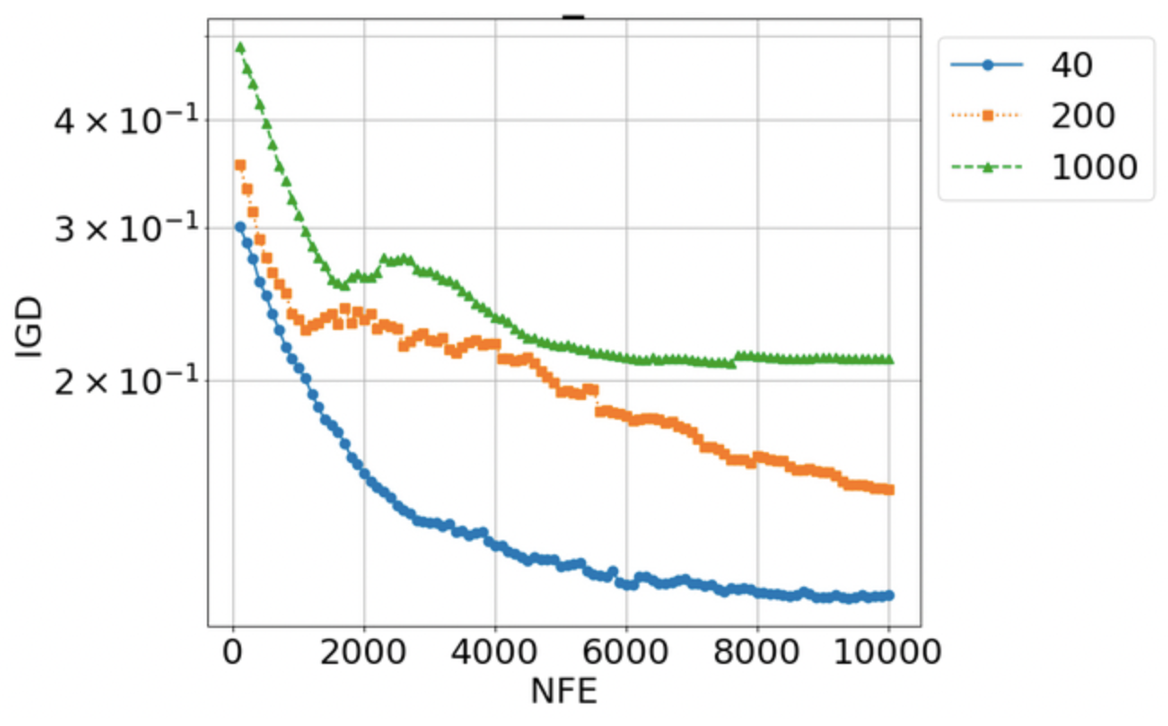
\includegraphics[width=0.5\linewidth]{img/fig1.png}
             \setlength{\abovecaptionskip}{0mm}
  \setlength{\belowcaptionskip}{0mm}
    \caption{設計変数の違いによる評価値の推移図}
\label{fig:nsgaiii}
\end{center}
\end{figure}
\vspace{-1.5zh}
\section{主成分分析を用いた進化計算手法}
\subsection{主成分分析(POD)について}
\vspace{-1.0zh}
主成分分析とは
%元のデータ(データは定量化できない質的変数ではなく量的変数である必要がある)から新しい変数を作ることまた,情報を減らさずに次元を減らす方法である.
元情報n次元の量的変数$x=(x_1,x_2,\cdots ,x_n)$が存在する場合、ある係数を掛け合わせて,新たな$x$の特徴を表した値 $y$(これを主成分という)を求めること,またその主成分を新たな変数として$X$の次元を減らす操作のことである.主成分$y$は$x$の線型結合和で次のように表すことができる.
\begin{eqnarray}
  y&=&w_1x_1+w_2x_2+\cdots+w_px_p
\end{eqnarray}
係数$w=(w_1,w_2,\cdots ,w_n)$を求める際には$x$に関する固有方程式を解く必要がある.
\vspace{-1.5zh}
\subsection{進化計算における主成分分析を用いた設計変数の次元削減の適用}
\vspace{-1.0zh}
本研究では進化計算の新たな個体を生成する部分に工夫を施したものとなっている.新たな個体を生成する際に解$X$を主成分分析を用いてより次元の小さい$X^{\prime}$に変換して交叉を行う.
新たに提案する手法についての流れを以下に示す.
\vspace{-1.5zh}
\begin{enumerate}
  \item 最初に乱数で個体群を生成する,
  \item 個体群が環境に適しているかどうかの評価をする
  \item 2.で評価した個体群から必要な数の個体を選択し,親個体群$P$を生成する
  \item 累積非劣解と親個体群に対して,主成分分析を行い、寄与率の合計が$95\%$を超えるまでの固有ベクトルを行列$W$とする.付随して$W$の逆行列$W^{\prime}$を求める.
  \item まず、親個体に$W$を用いて主成分へと変換し次元削減を行い$P^{\prime}$を生成する.その後$P^{\prime}$に交叉を行い新たな個体を生成、生成した個体を$W^{\prime}$で元の次元に戻し個体$Q$を生成.個体$Q$に突然変異を行い、子個体を生成する
  \item 生成した子個体群に対して環境に適しているかどうかの評価をする
  \item 計算は事前に与えられた条件(世代数や関数評価回数)を満たすと終了する.満たしていない場合,評価に応じて選択・淘汰を行う.選ばれた個体は次世代の親個体となり,4へ戻り同様の流れを繰り返すことによって環境に適した個体に進化していく.
\end{enumerate}
\section{計算条件}
設計変数の次元削減を用いた進化計算手法を結果として示す.以降,テスト問題にDTLZ2,計算手法にNSGA-IIを使用した結果を代表例として示す.またその他含め計算条件は表3.1に示したものになる.
\begin{table}[h]
\begin{center}
\begin{tabular}{cc}
\begin{minipage}{1\hsize}
\begin{center}
\caption{計算条件}
\label{tb::dataset}
\begin{tabular}{|c|c|}
\hline
テスト問題&DTLZ2 \\
\hline
進化計算手法&NSGA-II\\
\hline
親個体選択手法&ランダム選択,トーナメント選択\\
\hline
交叉手法&SBX\\
\hline
突然変異手法&polynomical mutation\\
\hline
目的数&4\\
\hline
設計変数&4\\
\hline
集団サイズ&100\\
\hline
世代数&10\\
\hline
試行回数&10\\
\hline
\end{tabular}
\end{center}
\end{minipage}
\end{tabular}
\end{center}
\end{table}
\vspace{-1.0zh}
\newpage
\section{結果と考察}
図4.1は,横軸を関数評価回数NFE、縦軸を解の評価指標値として評価指標値の推移図を表す.GDは解の収束性,IGDとHVは解の収束性と多様性を測る事ができる評価指標であり、GDとIGDに関しては値が小さいほど,HVに関しては値が大きいほど良い解とされる.また図4.2では横軸をNFE、縦軸を寄与率の合計が$95\%$を超えるまで抽出された主成分の数を表している.
\begin{figure}[htbp]
  \begin{center}
  \subfigure[GDの計算]{
    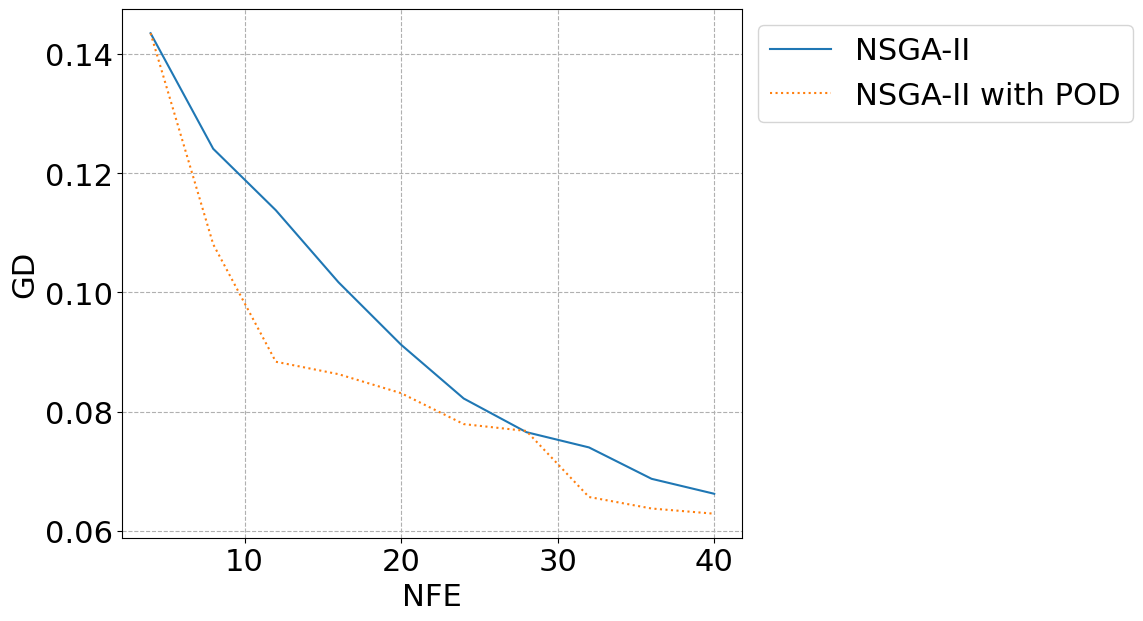
\includegraphics[width=0.45\linewidth]{img/4val-4pop-10gen-gd.png}
    \label{fig:dtlz3_credit1}
    }
     \subfigure[IGDの計算]{
    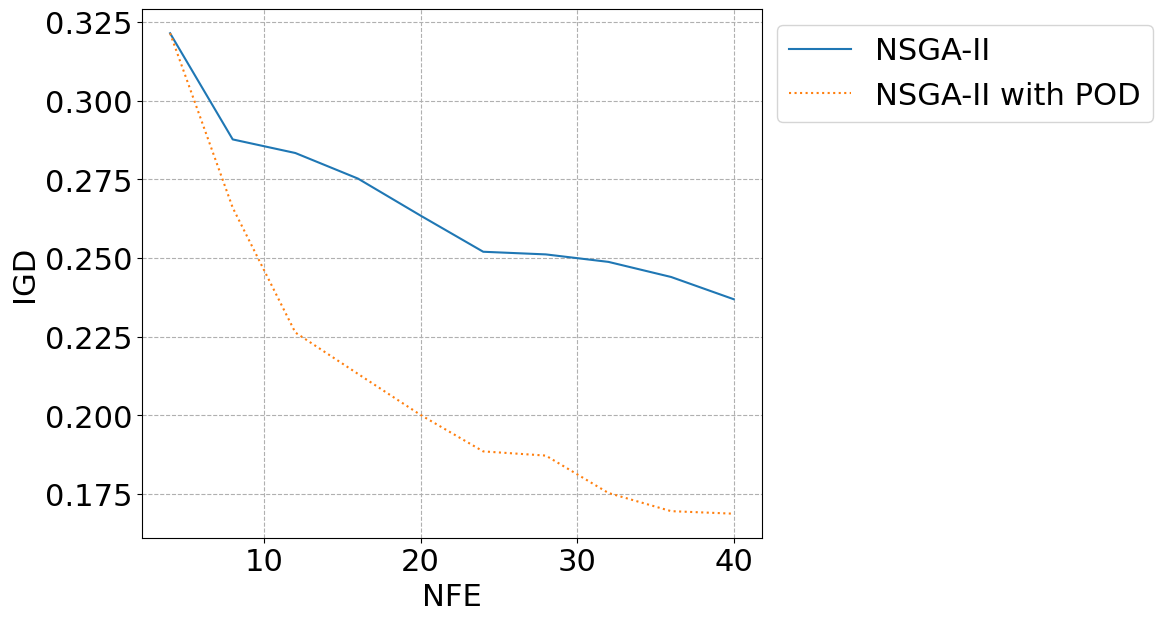
\includegraphics[width=0.45\linewidth]{img/4val-4pop-10gen-igd.png}
    \label{fig:dtlz3_credit2}
    }
    \subfigure[HVの計算]{
    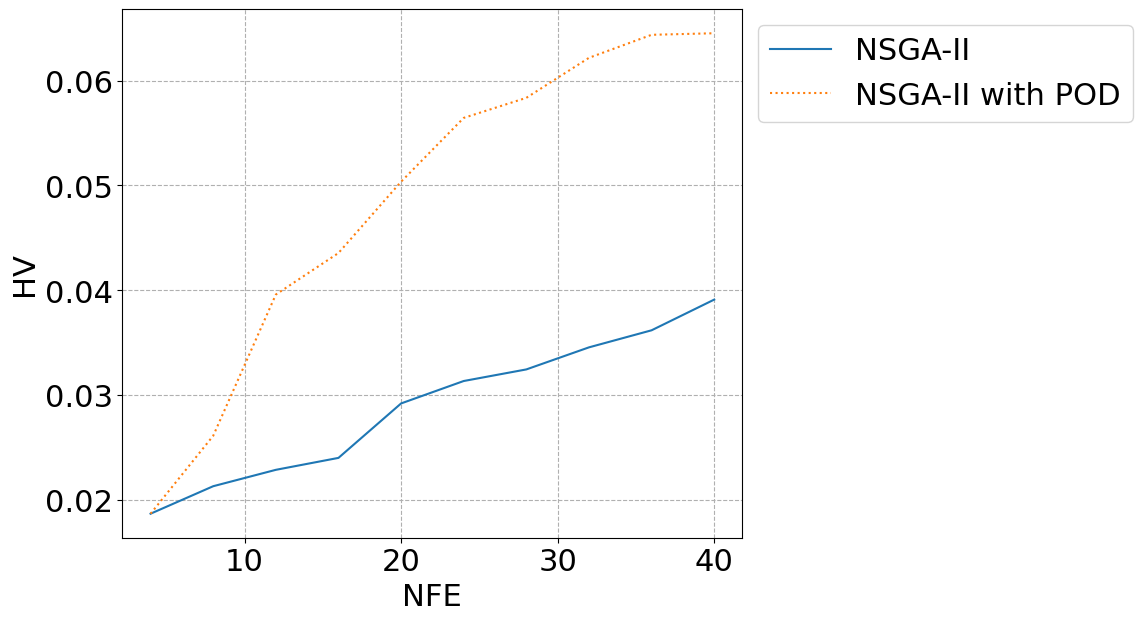
\includegraphics[width=0.45\linewidth]{img/4val-4pop-10gen-hv.png}
    \label{fig:dtlz3_credit1_improve}
    }
                \setlength{\abovecaptionskip}{0mm}
    \setlength{\belowcaptionskip}{0mm}
      \caption{各評価指標による比較}
  \label{fig:ranking}
  \end{center}
\end{figure}
\begin{figure}[htbp]
\begin{center}
  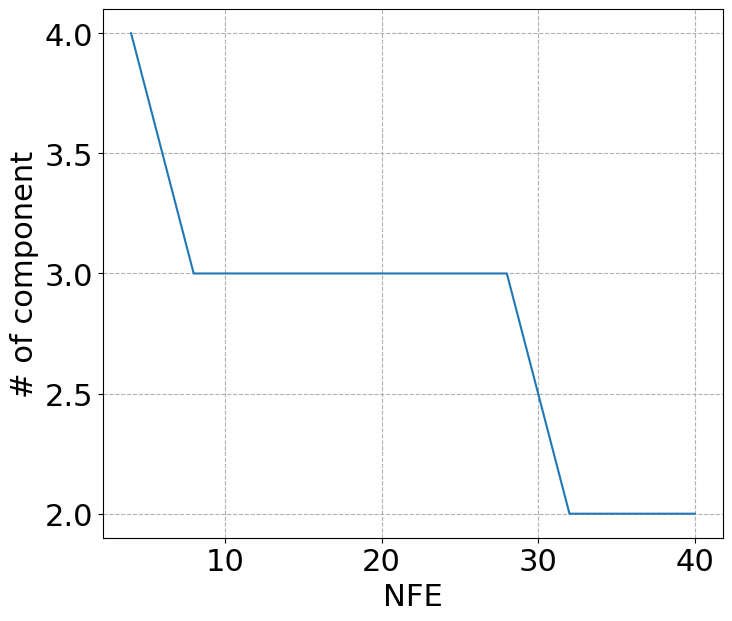
\includegraphics[width=0.3\linewidth]{img/4val-4pop-10gen-component-hist.png}
             \setlength{\abovecaptionskip}{0mm}
  \setlength{\belowcaptionskip}{0mm}
    \caption{計算中に使われる主成分の数}
\label{fig:nsgaiii}
\end{center}
\end{figure}
図4.1から考察する.全ての評価指標においてPODを導入したNSGA-II(NSGA-II/P)の方が優れていたのがわかる.また少ないNFEからもNSGA-II/Pの方が優れている.これは少ない計算回数でより良い解が求められていることを示す.さらに、GDでは計算終了時での差が見られないことから今回の計算では収束性に関して最終的には優劣を明らかに確認することはできなかったが、IGDとHVにおいて大きな差があることから収束性には小さなさ違いしか示されなかった反面、多様性においてとても優れていると結論づけることができる.次に、図4.2に注目する.最初は寄与率が$95\%$を超えるように主成分を抽出すると4つ抽出されていた.これは全ての主成分を用いていたことがわかる.一方で計算が進むごとに抽出される主成分が少なくなっていることから、設計変数の特徴を段々と掴むことに成功しているのがわかる.これは母集団だけでなく累積非列解を使い主成分分析を行うことにより、計算を重ねるごとに設計変数についての情報を取得できていることを裏付ける.
\begin{comment}
\begin{figure}[htbp]
  \begin{center}
  \subfigure[各評価値の計算]{
     \subfigure[GDの計算]{
    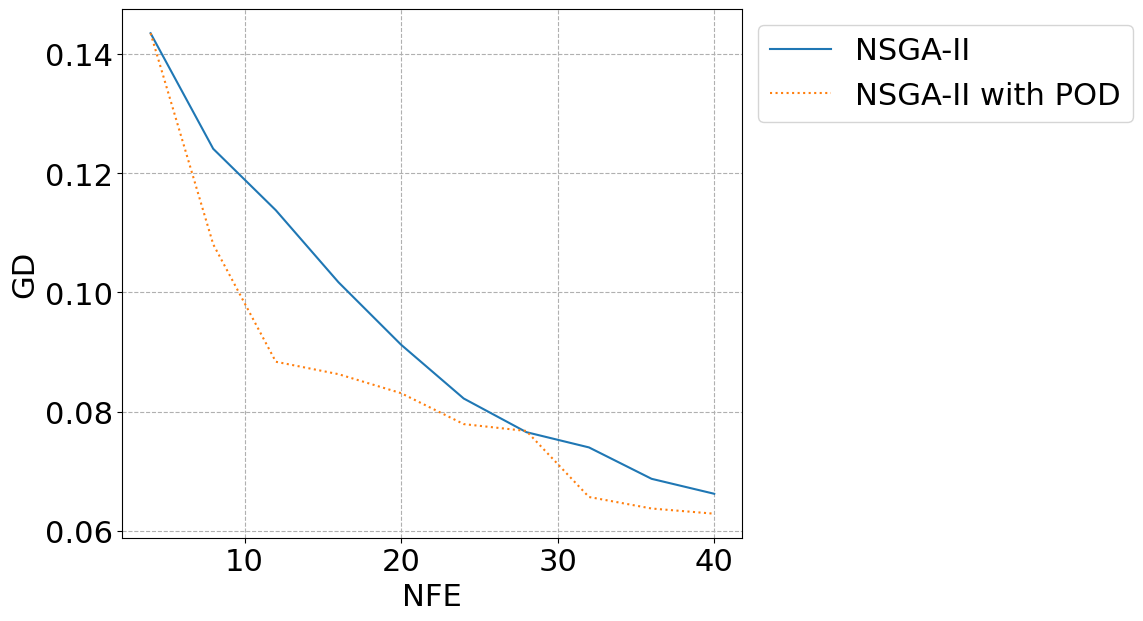
\includegraphics[width=0.3\linewidth]{img/4val-4pop-10gen-gd.png}
    \label{fig:dtlz3_credit2}
    }
    \subfigure[IGDの計算]{
    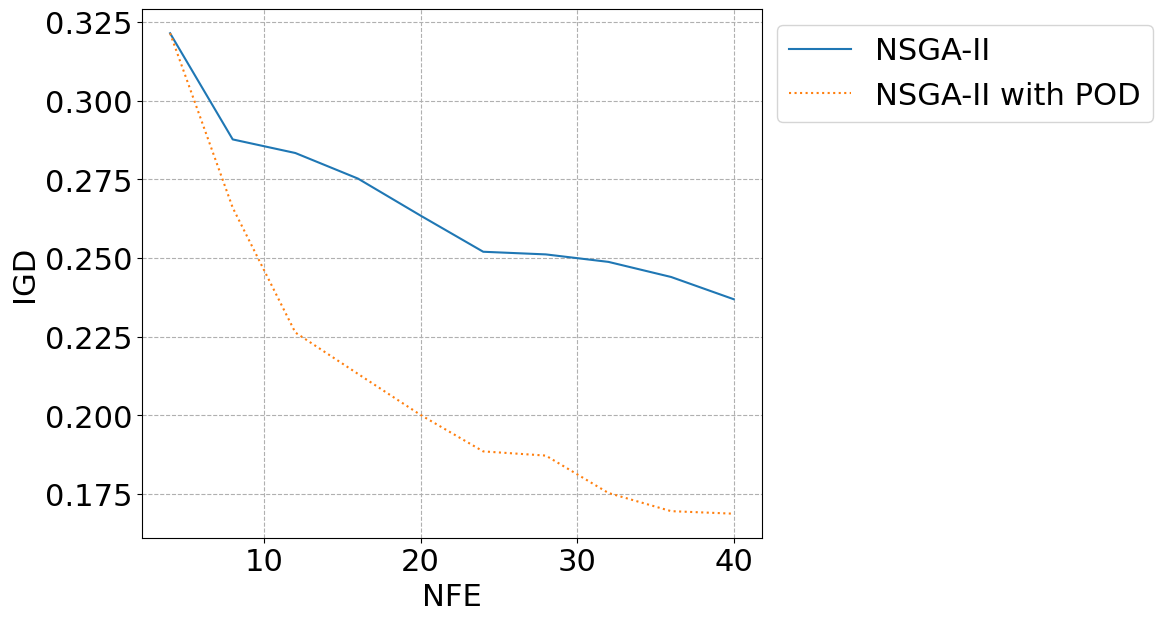
\includegraphics[width=0.3\linewidth]{img/4val-4pop-10gen-igd.png}
    \label{fig:dtlz3_credit1_improve}
    }
    \subfigure[HVの計算]{
    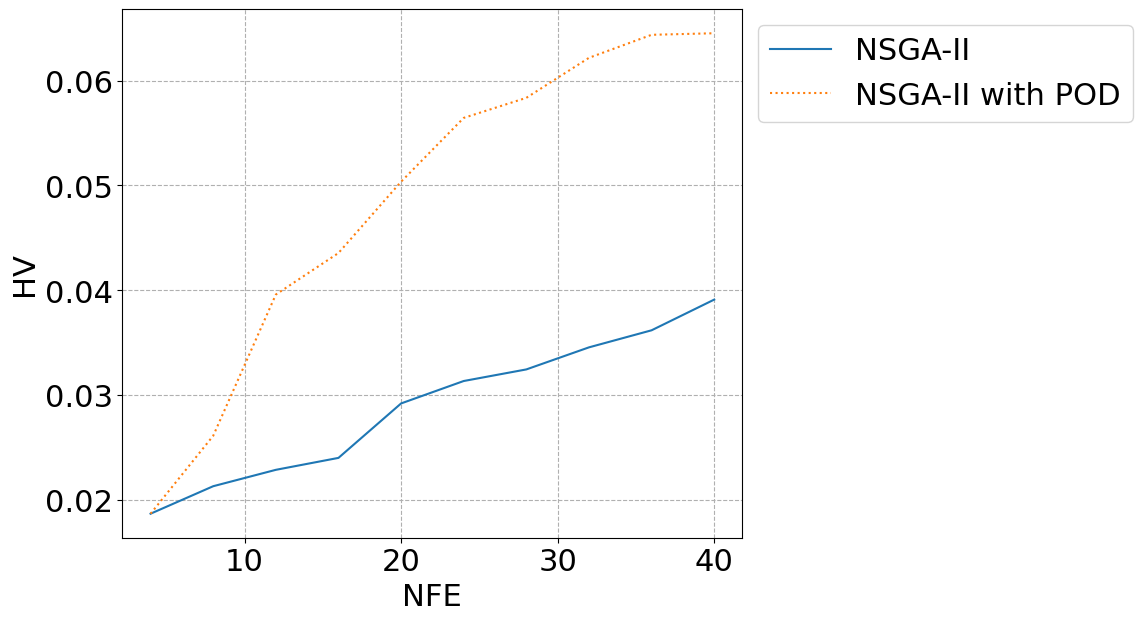
\includegraphics[width=0.3\linewidth]{img/4val-4pop-10gen-hv.png}
    \label{fig:dtlz3_credit1_improve}
    }
                \setlength{\abovecaptionskip}{0mm}
    \setlength{\belowcaptionskip}{0mm}
      \caption{各評価値の計算}
  \label{fig:ranking}
  \end{center}
\end{figure}
\end{comment}
\section{まとめと今後の課題}
\vspace{-1.0zh}
今回の例では、少ない設計変数と母集団サイズでの紹介になっている.これは計算量が何らかの原因で大きくなっているためであり、今後LSGO問題に対応するべく原因を解明しさまざまなテスト問題に対して本研究を進めて行きたい.
\vspace{-1.0zh}
\begin{thebibliography}{99}
  {\fontsize{10pt}{10pt}\selectfont
\bibitem{Do}鐘 睿,高木 英行."大規模最適化問題へのスパースモデリング導入"pp.1-, 2021-03-04. 進化計算学会
\bibitem{Sato1}佐藤 寛之,石渕 久生."進化型多数目的最適化の現状と課題"オペレーションズリサーチ学会2017 年 3 月号
\bibitem{Deb1}K. Deb and K. Saxena.“Searching for Paretooptimal solutions through dimensionality reduction for
certain large-dimensional multi-objective optimization
problems,” In Proeedings of 2006 IEEE Congress on
Evolutionary Computation (CEC 2006), pp. 3353–
3360, 2006.
\bibitem{HSato}H. Sato, H. Aguirre and K. Tanaka, “Controlling
dominance area of solutions and its impact on the performance of MOEAs,” International Conference on Evolutionary Multi-Criterion Optimization
EMO 2007: Evolutionary Multi-Criterion Optimization pp 5-20
\bibitem{Yo}余 俊, 高木 英行,“強制約条件付き最適化問題の2段階探索”進化計算シンポジウム 2017, 北海道茅部郡森町,pp.38-41 (2017年12月9-10日)
\bibitem{Chai}Chai T, Jin Y, Sendhoff B,"Evolutionary complex
engineering optimization" Opportunities and challenges. IEEE Computational Intelligence Magazine2013, 8(3):12-15.
}
\end{thebibliography}

\end{document}
